\chapter{Corrosie en bescherming}\label{ch:b2:corrosion}

Laat een druppel zout water liggen op een schoon stuk staal. Na een dag is het metaal
in het midden van de druppel aangevreten, terwijl de roest zich in een ring bij de
rand heeft gevormd, waar de zuurstof van de lucht oplost. Het ijzer lost op waar
het minste zuurstof is, en de zuurstof wordt gereduceerd waar er het meeste is: de druppel
is een cel die niemand gebouwd heeft, kortgesloten via het metaal zelf. Dit
hoofdstuk leest corrosie af op \omterm{def:b2:current-potential-curves:ie-curve}{stroom-potentiaalkrommen}, verklaart waarom een
bekraste gegalvaniseerde plaat niet roest en een bekrast conservenblik wel, en
ontwerpt de bescherming van een ingegraven pijpleiding.

\begin{recall}
Het deel van jaar~1: potentiaal-pH-diagrammen van metalen en hun immuniteitsgebieden,
corrosie en \omterm{def:b2:corrosion:passivation}{passivering} (``of een laag beschermt, is een kinetische kwestie'').
\Cref{ch:b2:current-potential-curves}: \omterm{def:b2:current-potential-curves:ie-curve}{stroom-potentiaalkrommen},
\omterm{def:b2:current-potential-curves:limiting-current}{grensstromen}. \Cref{ch:b2:batteries-electrolysis}: de \omterm{def:b2:batteries-electrolysis:mixed-potential}{gemengde potentiaal}. Het
schoolboek: corrosie, roest, verzinken.
\end{recall}

\begin{omfigure}
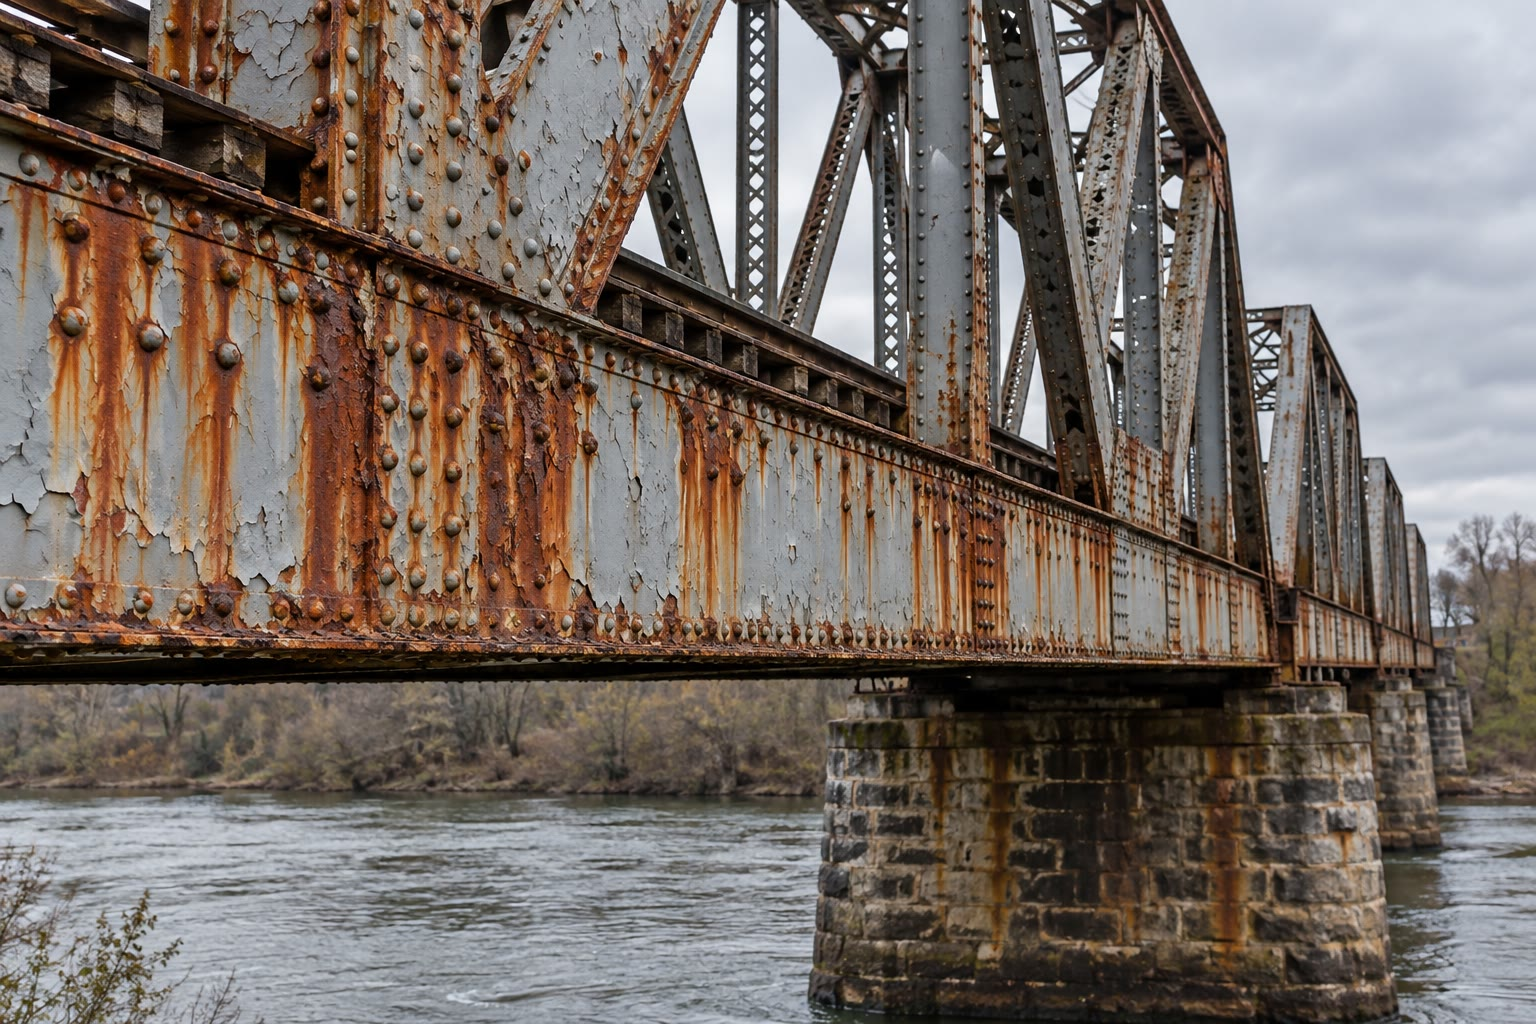
\includegraphics[width=0.62\linewidth]{images/book3/ai/b2-12-rusty-bridge.jpg}

{\small Een oude geklonken spoorbrug. Roeststrepen lopen naar beneden vanaf de klinknagels
en de voegen, waar water en zuurstof het langst blijven en de verf het eerst
het begeeft.}
\end{omfigure}

\section{Natte corrosie als kortgesloten cel}

In water met opgeloste zuurstof wordt ijzer geoxideerd, \ce{Fe -> Fe^2+ + 2e-},
en de elektronen worden op hetzelfde stuk metaal opgenomen door de reductie van
dizuurstof, \ce{O2 + 2H2O + 4e- -> 4OH-} (in zuur milieu ook door \ce{2H+ + 2e- -> H2}). De
ijzer(II)-ionen en de hydroxide-ionen ontmoeten elkaar in het water, en verdere oxidatie door
de lucht maakt van hun neerslag roest, een gehydrateerd ijzer(III)oxide.

\begin{definition}[Uniforme corrosie]\label{def:b2:corrosion:uniform}
\emph{Uniforme corrosie}\index{uniforme corrosie} is de corrosie van een metaal
waarvan de oxidatie en de reductie van de oxidator plaatsvinden op plekken die
gelijkmatig over zijn oppervlak verspreid zijn. De \emph{corrosiepotentiaal}\index{corrosiepotentiaal}
is de \omterm{def:b2:batteries-electrolysis:mixed-potential}{gemengde potentiaal} die het metaal dan aanneemt, en de
\emph{corrosiestroom}\index{corrosiestroom} de \omterm{def:b2:current-potential-curves:ie-curve}{anodische stroom} van de
oxidatie van het metaal bij die potentiaal.
\end{definition}

\begin{omfigure}
\begin{tikzpicture}
\begin{axis}[omie, width=0.82\linewidth, height=5.6cm, xmin=-1.1, xmax=0.5,
  ymin=-1.6, ymax=1.6, xlabel={$E$}, ylabel={$i$}, clip=true, clip mode=individual,
  axis y line=left]
\addplot[omanodic] table[x=E, y=i] {figdata/out/bachelor-2-ie-curves-i-Fe.dat};
\addplot[omcathodic] table[x=E, y=i] {figdata/out/bachelor-2-ie-curves-i-O2.dat};
\addplot[omcathodic, densely dashed] table[x=E, y=i, y expr=-\thisrow{i}] {figdata/out/bachelor-2-ie-curves-i-O2.dat};
\draw[densely dotted] (axis cs:-0.394,-1.0) -- (axis cs:-0.394,1.0);
\fill (axis cs:-0.394,1.0) circle (1.4pt);
\node[font=\scriptsize, anchor=south east] at (axis cs:-0.40,1.02) {$i_{\text{corr}}$};
\node[font=\scriptsize, anchor=north west] at (axis cs:-0.39,-0.03) {$E_{\text{corr}}$};
\node[font=\scriptsize, omThm, anchor=west] at (axis cs:-0.35,1.4) {\ce{Fe} $\to$ \ce{Fe^2+}};
\node[font=\scriptsize, omDef, anchor=north west] at (axis cs:-0.75,-1.05) {\ce{O2} $\to$ \ce{OH-}, diffusieplateau};
\end{axis}
\end{tikzpicture}

{\small Het evansdiagram van ijzer in belucht neutraal water (modelkrommen). De
kathodische kromme van dizuurstof is ook naar boven gespiegeld getekend (gestreept): de
\omterm{def:b2:corrosion:uniform}{corrosiepotentiaal} ligt waar ze de anodische kromme van ijzer snijdt. Omdat de
reductie van dizuurstof daar haar diffusieplateau bereikt heeft, is de \omterm{def:b2:corrosion:uniform}{corrosiestroom}
gelijk aan de \omterm{def:b2:current-potential-curves:limiting-current}{grensstroom} van zuurstof: roeren of beluchten van het water
laat ijzer sneller corroderen.}
\end{omfigure}

\begin{proposition}[Corrosiesnelheid]\label{prop:b2:corrosion:rate}
Een metaal met molaire massa $M$ en dichtheid $\rho$, geoxideerd met $n$ elektronen per
atoom onder een corrosiestroomdichtheid $j_{\text{corr}}$ (stroom per eenheid oppervlakte),
verliest per eenheid oppervlakte en tijd de massa $j_{\text{corr}}M/(nF)$, dus een
dikte
\[
  \frac{de}{dt} = \frac{j_{\text{corr}}\,M}{nF\rho} .
\]
\end{proposition}

\begin{proof}
Volgens \cref{prop:b2:current-potential-curves:current-rate} oxideert de anodische
stroomdichtheid $j_{\text{corr}}$ per eenheid oppervlakte en tijd $j_{\text{corr}}/(nF)$ mol metaal;
vermenigvuldig met $M$ voor de massa en deel door $\rho$ voor de dikte.
\end{proof}

\begin{example}[IJzer bij \qty{10}{\micro A/cm^2}]\label{ex:b2:corrosion:rate}
Met $j = \qty{0.10}{A/m^2}$, $M = \qty{55.845}{g/mol}$, $n = 2$, $\rho =
\qty{7.87}{g/cm^3}$: $de/dt = 0.10 \times 55.845/(2 \times 96\,485 \times 7.87
\times 10^6) = \qty{3.7e-12}{m/s}$, dus \qty{0.12}{mm} per jaar.
% ledger: aw:Fe, rho:Fe, const:F
\end{example}

\section{Differentiële corrosie}

\begin{definition}[Differentiële corrosie]\label{def:b2:corrosion:differential}
\emph{Differentiële corrosie}\index{differentiele corrosie@differentiële corrosie} is een corrosie
waarbij de anodische en de kathodische plekken gescheiden zijn, zodat het metaal
bij voorkeur op de anodische plekken geoxideerd wordt. Het is \emph{galvanische
corrosie}\index{galvanische corrosie} wanneer twee verschillende metalen in elektrisch
contact hetzelfde elektrolyt delen, en \emph{differentiële
beluchting}\index{differentiele beluchting@differentiële beluchting} wanneer één metaal blootgesteld is aan water met
verschillende zuurstofgehalten.
\end{definition}

\begin{proposition}[Twee metalen in contact]\label{prop:b2:corrosion:galvanic}
Wanneer twee metalen in elektrisch contact in hetzelfde beluchte water dompelen, nemen ze
één enkele \omterm{def:b2:batteries-electrolysis:mixed-potential}{gemengde potentiaal} aan. Het metaal met de laagste \omterm{def:b2:corrosion:uniform}{corrosiepotentiaal}
wordt de anode en corrodeert sneller dan alleen; het andere wordt een kathode,
waarop dizuurstof gereduceerd wordt, en is beschermd.
\end{proposition}

\begin{proof}
Verbonden door een geleider met verwaarloosbare weerstand hebben de twee metalen dezelfde
potentiaal, waarbij de som van alle anodische stromen gelijk is aan min de som van
alle kathodische stromen. De anodische kromme van het minder edele metaal stijgt eerst;
bij de gemeenschappelijke potentiaal voert ze bijna de hele \omterm{def:b2:current-potential-curves:ie-curve}{anodische stroom}, en de
zuurstof wordt gereduceerd op het hele bevochtigde oppervlak, het edelere metaal inbegrepen,
waarvan de eigen \omterm{def:b2:current-potential-curves:ie-curve}{anodische stroom} daar verwaarloosbaar is.
\end{proof}

\begin{omfigure}
\begin{tikzpicture}
\begin{axis}[omie, width=0.82\linewidth, height=5.6cm, xmin=-1.1, xmax=0.5,
  ymin=-2.4, ymax=2.4, xlabel={$E$}, ylabel={$i$}, clip=true, clip mode=individual,
  axis y line=left]
\addplot[omanodic] table[x=E, y=i] {figdata/out/bachelor-2-ie-curves-i-Fe.dat};
\addplot[omanodic, densely dashed] table[x=E, y=i] {figdata/out/bachelor-2-ie-curves-j-Zn.dat};
\addplot[omcathodic] table[x=E, y=i] {figdata/out/bachelor-2-ie-curves-i-O2.dat};
\addplot[omcathodic, densely dashed] table[x=E, y=i] {figdata/out/bachelor-2-ie-curves-j-O2Cu.dat};
\fill (axis cs:-0.394,1.0) circle (1.4pt);
\fill (axis cs:-0.794,1.0) circle (1.4pt);
\fill (axis cs:-0.366,2.0) circle (1.4pt);
\draw[densely dotted] (axis cs:-1.1,1.0) -- (axis cs:-0.394,1.0);
\draw[densely dotted] (axis cs:-1.1,2.0) -- (axis cs:-0.366,2.0);
\node[font=\scriptsize, anchor=south west] at (axis cs:-0.38,0.95) {ijzer alleen};
\node[font=\scriptsize, anchor=west] at (axis cs:-0.35,2.0) {ijzer + koper};
\node[font=\scriptsize, anchor=south east] at (axis cs:-0.80,1.05) {ijzer + zink};
\node[font=\scriptsize, omThm, anchor=north west] at (axis cs:-0.98,0.75) {zink};
\node[font=\scriptsize, omThm, anchor=north west] at (axis cs:-0.55,0.75) {ijzer};
\node[font=\scriptsize, omDef, anchor=north east] at (axis cs:0.45,-2.05) {\ce{O2} op ijzer + koper};
\node[font=\scriptsize, omDef, anchor=north east] at (axis cs:0.45,-1.05) {\ce{O2} op ijzer};
\end{axis}
\end{tikzpicture}

{\small IJzer gekoppeld aan andere metalen (modelkrommen). Met zink zakt de gemeenschappelijke
potentiaal tot waar zink de \omterm{def:b2:current-potential-curves:ie-curve}{anodische stroom} voert: ijzer is beschermd,
zink corrodeert. Met koper verdubbelt het kathodische oppervlak voor zuurstof: ook de
\omterm{def:b2:corrosion:uniform}{corrosiestroom} van ijzer verdubbelt.}
\end{omfigure}

\begin{proposition}[Differentiële beluchting]\label{prop:b2:corrosion:aeration}
Op een metaal dat blootgesteld is aan water met verschillende zuurstofgehalten, is de minst beluchte
zone anodisch en corrodeert ze; de best beluchte zone is kathodisch.
\end{proposition}

\begin{proof}
Waar het zuurstofgehalte hoger is, heeft het koppel \ce{O2}/\ce{OH-} een hogere
nernstpotentiaal en een grotere \omterm{def:b2:current-potential-curves:limiting-current}{grensstroom}: de kathodische kromme ligt hoger
en reikt verder. Het metaal, één enkele geleider, neemt één potentiaal aan;
de grote \omterm{def:b2:current-potential-curves:ie-curve}{kathodische stroom} die in de beluchte zone beschikbaar is, moet gecompenseerd worden door een
\omterm{def:b2:current-potential-curves:ie-curve}{anodische stroom}, die loopt waar het metaal geoxideerd kan worden met weinig
concurrentie van de zuurstofreductie: in de slecht beluchte zone. De oxidatie
concentreert zich daar.
\end{proof}

\begin{omfigure}
\begin{tikzpicture}[font=\small, >={Stealth}]
  \fill[black!20] (-4.2,-0.7) rectangle (4.2,0);
  \node[font=\scriptsize] at (3.7,-0.35) {staal};
  \fill[omDef!15] (-3.4,0) .. controls (-2.9,2.2) and (2.9,2.2) .. (3.4,0) -- cycle;
  \draw[thick, omDef] (-3.4,0) .. controls (-2.9,2.2) and (2.9,2.2) .. (3.4,0);
  \fill[omProp!80] (-0.7,0) arc[start angle=180, end angle=360, x radius=0.7, y radius=0.22] -- cycle;
  \fill[brown!70!black] (-1.9,0.12) ellipse (0.45 and 0.11);
  \fill[brown!70!black] (1.9,0.12) ellipse (0.45 and 0.11);
  \node[font=\scriptsize, align=center] at (0,2.45) {\ce{O2} uit de lucht};
  \draw[->, thick, omDef] (-1.0,2.25) -- (-2.6,0.35);
  \draw[->, thick, omDef] (1.0,2.25) -- (2.6,0.35);
  \node[font=\scriptsize, align=center, anchor=east] at (-4.1,1.3) {kathode\\ (rand)};
  \draw[->, thin] (-4.1,1.3) -- (-3.05,0.12);
  \node[font=\scriptsize, align=center, anchor=west] at (4.1,1.3) {roestring};
  \draw[->, thin] (4.1,1.3) -- (2.3,0.2);
  \draw[->, omThm] (-0.4,-0.3) .. controls (-1.2,-0.5) and (-2.4,-0.5) .. (-3.0,-0.15);
  \draw[->, omThm] (0.4,-0.3) .. controls (1.2,-0.5) and (2.4,-0.5) .. (3.0,-0.15);
  \draw[->, thin] (0,-1.05) -- (0,-0.25);
  \node[font=\scriptsize, anchor=north] at (0,-1.05) {anode (midden): \ce{Fe -> Fe^2+ + 2e-}};
  \node[font=\scriptsize, omThm, anchor=north] at (0,-1.45) {elektronen stromen door het staal naar de rand};
  \node[font=\scriptsize, anchor=north] at (0,-1.85) {kathode (rand): \ce{O2 + 2H2O + 4e- -> 4OH-}};
\end{tikzpicture}

{\small De druppel van Evans op staal, schematisch. Zuurstof lost op aan het oppervlak en
bereikt het metaal vooral bij de dunne rand van de druppel, die de
kathode wordt; het midden, verstoken van zuurstof, is de anode en wordt aangevreten. De
ijzer(II)-ionen en de hydroxide-ionen ontmoeten elkaar daartussen, waar de roest
als een ring neerslaat.}
\end{omfigure}

Hetzelfde mechanisme tast spleten aan, de delen van een constructie onder een afzetting
of een pakking, en een stalen paal in zee net onder de waterlijn, waar
het water minder belucht is dan aan het oppervlak.

\begin{method}[Een corrosie diagnosticeren]\label{met:b2:corrosion:diagnose}
\begin{enumerate}
  \item Som de metalen in contact en het elektrolyt op; controleer of ze
        elektrisch verbonden zijn.
  \item Bij twee metalen is het metaal met de laagste \omterm{def:b2:corrosion:uniform}{corrosiepotentiaal} (meestal de
        laagste standaardpotentiaal) de anode.
  \item Zoek bij één metaal de minst beluchte zones (spleten, onder afzettingen,
        de bodem van een druppel): die zijn anodisch.
  \item De snelheid wordt bepaald door de kathodische reactie (zuurstofaanvoer, kathodeoppervlak):
        een kleine anode op een grote kathode corrodeert snel.
\end{enumerate}
\end{method}

\section{Passivering}

\begin{definition}[Passivering]\label{def:b2:corrosion:passivation}
\emph{Passivering}\index{passivering} is de sterke daling van de corrosiesnelheid
van een metaal wanneer het bedekt wordt door een dunne, compacte, hechtende laag van zijn
oxide, de \emph{passieve film}\index{passieve film}, die het van de
oplossing scheidt. Een metaal in deze toestand heet passief.
\end{definition}

\begin{proposition}[Het passieve plateau]\label{prop:b2:corrosion:passivity}
De anodische kromme van een passiveerbaar metaal stijgt vanaf zijn \omterm{def:b2:corrosion:uniform}{corrosiepotentiaal},
bereikt een piek, en daalt dan tot een kleine, bijna constante passieve stroom over een
potentiaalgebied, voordat ze bij hoge potentialen opnieuw stijgt (transpassief
gebied: oxidatie van de film of van water). De passieve toestand kan plaatselijk
doorbroken worden, bijvoorbeeld door chloride-ionen, wat putten geeft.
\end{proposition}

\begin{proof}[Redenering]
Bij kleine \omterm{def:b2:current-potential-curves:overpotential}{overspanningen} lost het blote metaal steeds sneller op. Voorbij een
drempel wordt het oxide stabiel aan het oppervlak (het passiveringsgebied van
het potentiaal-pH-diagram) en vormt het een film waardoor ionen slechts traag bewegen: de
stroom stort in tot die kleine flux. Bij hoge potentialen wordt de film zelf
geoxideerd tot oplosbare deeltjes, of wordt water erop geoxideerd. Chloride-ionen, klein
en sterk complexerend, kunnen de film op zwakke plekken oplossen, waar het blote
metaal dan corrodeert als een kleine anode tegenover een enorme passieve kathode. De
vorm van de kromme is hier een model.
\end{proof}

\begin{omfigure}
\begin{tikzpicture}
\begin{axis}[omie, width=0.82\linewidth, height=5.4cm, xmin=-0.7, xmax=1.5,
  ymin=-0.1, ymax=1.3, xlabel={$E$}, ylabel={$i$}, clip=true, clip mode=individual,
  axis y line=left]
\addplot[omanodic] table[x=E, y=i] {figdata/out/bachelor-2-ie-curves-k.dat};
\node[font=\scriptsize, anchor=south] at (axis cs:-0.33,1.0) {actief};
\node[font=\scriptsize, anchor=south] at (axis cs:0.5,0.06) {passief plateau};
\node[font=\scriptsize, anchor=east] at (axis cs:1.25,0.9) {transpassief};
\draw[<-, thin] (axis cs:-0.2,0.55) -- (axis cs:0.15,0.7) node[right, font=\scriptsize] {film ontstaat};
\end{axis}
\end{tikzpicture}

{\small Anodische kromme van een passiveerbaar metaal (model). De stroom, groot zolang
het blote metaal oplost, stort in wanneer de \omterm{def:b2:corrosion:passivation}{passieve film} ontstaat, en blijft
klein over een breed potentiaalgebied vóór de transpassieve stijging.}
\end{omfigure}

Roestvaste staalsoorten bevatten genoeg chroom om een \omterm{def:b2:corrosion:passivation}{passieve film} van chroomoxide te vormen
die zich in lucht zelf herstelt; aluminium wordt beschermd door zijn oxidefilm, wat
een metaal dat in de reeks ver onder waterstof staat, bruikbaar maakt voor raamkozijnen en
drankblikjes. Koper wordt groen in de open lucht: de patina is een laag
basische kopersouten die verdere aantasting vertraagt.

\begin{omfigure}
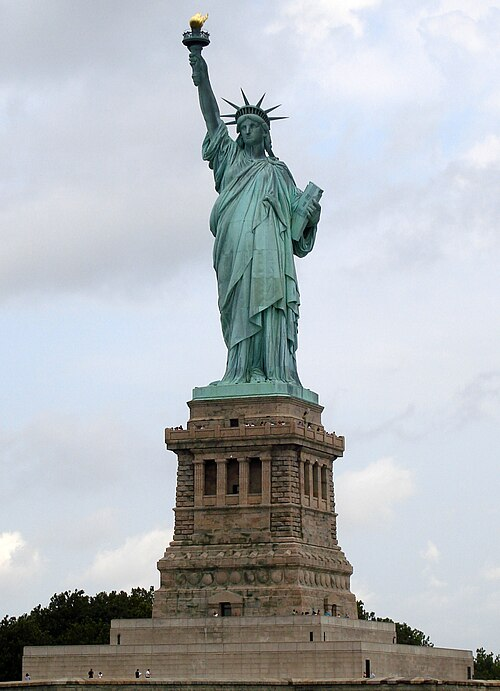
\includegraphics[width=0.32\linewidth]{images/book3/liberty.jpg}

{\small Een koperen beeld van meer dan een eeuw oud: zijn huid van dun koperblik
is groen geworden, bedekt met een patina van basische kopersouten die het
metaal eronder beschermt. (Foto: Elcobbola, publiek domein, Wikimedia Commons.)}
\end{omfigure}

\section{Bescherming}

Corrosie wordt bestreden door het metaal van water en zuurstof te scheiden (verf,
kunststof, email, of een laag van een ander metaal), door het milieu te veranderen
(zuurstof verwijderen, inhibitoren toevoegen die op het metaal adsorberen), of door de
potentiaal van het metaal naar zijn immuniteitsgebied te verschuiven.

\begin{definition}[Kathodische bescherming]\label{def:b2:corrosion:protection}
\emph{Kathodische bescherming}\index{kathodische bescherming} verlaagt de potentiaal van een
metalen constructie tot haar oxidatie stopt, door er de kathode van een cel van te maken.
De cel kan gevormd worden met een \emph{opofferingsanode}\index{opofferingsanode},
een minder edel metaal (zink, magnesium, aluminiumlegeringen) dat met de
constructie verbonden is en in haar plaats verbruikt wordt, of aangedreven worden door een generator, bij
\emph{bescherming met opgedrukte stroom}\index{bescherming met opgedrukte stroom}, waarbij de
anode dan een inerte elektrode is die in de buurt is ingegraven.
\end{definition}

\begin{proposition}[Levensduur van een opofferingsanode]\label{prop:b2:corrosion:anode-life}
Een \omterm{def:b2:corrosion:protection}{opofferingsanode} met massa $m$ en molaire massa $M$, geoxideerd met $n$ elektronen
en een rendement $\eta$ (de fractie van het metaal die nuttige
stroom levert, terwijl de rest op zichzelf corrodeert), levert een stroom $I$ gedurende een tijd
\[
  t = \frac{\eta\,m\,nF}{M I} .
\]
\end{proposition}

\begin{proof}
De nuttige lading is $\eta\,(m/M)\,nF$; deel door de stroom.
\end{proof}

\begin{omfigure}
\begin{tikzpicture}[font=\small, >={Stealth}]
  \fill[brown!20] (-4.2,-2.4) rectangle (4.2,0);
  \draw[thick] (-4.2,0) -- (4.2,0);
  \node[font=\scriptsize, anchor=south west] at (-4.2,0) {bodem};
  \fill[black!40] (-3.5,-1.6) rectangle (3.5,-1.2);
  \node[font=\scriptsize, white] at (0,-1.4) {stalen buis (kathode)};
  % sacrificial anode
  \fill[black!65] (-3.2,-2.3) rectangle (-2.2,-1.95);
  \node[font=\scriptsize, anchor=north] at (-2.7,-2.3) {Mg-anode};
  \draw[thick] (-2.7,-1.95) -- (-2.7,-1.6);
  \draw[->, omProp, thick] (-2.2,-2.12) -- (-1.4,-1.7);
  \node[font=\scriptsize, omProp, anchor=west] at (-1.9,-2.2) {stroom in de bodem};
  % impressed current
  \draw[thick, rounded corners] (1.8,0.4) rectangle (3.2,1.2);
  \node[font=\scriptsize] at (2.5,0.8) {gelijkrichter};
  \fill[black!65] (3.4,-2.3) rectangle (3.9,-1.8);
  \node[font=\scriptsize, anchor=north] at (3.65,-2.3) {inerte anode};
  \draw[thick] (3.2,0.8) -- (3.65,0.8) -- (3.65,-1.8);
  \draw[thick] (1.8,0.8) -- (1.2,0.8) -- (1.2,-1.2);
  \node[font=\scriptsize, anchor=south] at (3.65,0.85) {$+$};
  \node[font=\scriptsize, anchor=south] at (1.2,0.85) {$-$};
  \node[font=\scriptsize, align=center] at (-2.7,0.8) {opofferingsanode};
  \node[font=\scriptsize, align=center] at (2.5,1.55) {opgedrukte stroom};
\end{tikzpicture}

{\small \omterm{def:b2:corrosion:protection}{Kathodische bescherming} van een ingegraven buis, schematisch. Links: een magnesiumanode,
met een draad aan de buis verbonden, corrodeert in haar plaats. Rechts: een gelijkrichter stuurt een
stroom van een inerte anode door de bodem naar de buis.}
\end{omfigure}

\begin{omfigure}
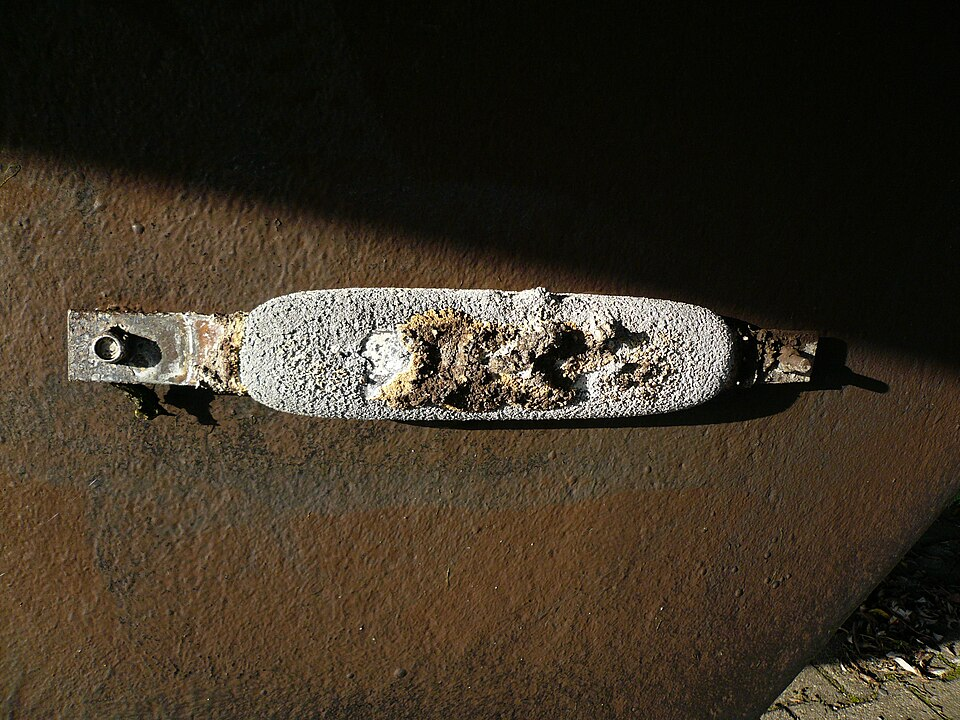
\includegraphics[width=0.5\linewidth]{images/book3/sacrificial-anode.jpg}

{\small Een \omterm{def:b2:corrosion:protection}{opofferingsanode} van zink, op de stalen romp van een boot geschroefd, na een
seizoen in het water: het zink is weggevreten, het staal eromheen is intact.
(Foto: Zwergelstern, CC BY-SA 3.0, Wikimedia Commons.)}
\end{omfigure}

\begin{omfigure}
\begin{tikzpicture}[font=\small, >={Stealth}, scale=1.35]
  \begin{scope}
    \fill[black!25] (0,0) rectangle (4,0.6);
    \fill[gray!55] (0,0.6) rectangle (1.7,0.8); \fill[gray!55] (2.3,0.6) rectangle (4,0.8);
    \fill[omDef!15] (0.8,0.8) .. controls (1.3,1.3) and (2.7,1.3) .. (3.2,0.8) -- (2.3,0.8) -- (2.3,0.6) -- (1.7,0.6) -- (1.7,0.8) -- cycle;
    \node[font=\scriptsize] at (2,-0.3) {gegalvaniseerd staal (zinklaag)};
    \node[font=\scriptsize, align=center] at (2,1.6) {zink corrodeert,\\ staal beschermd};
    \draw[->, omThm] (1.4,0.85) -- (1.8,0.65);
  \end{scope}
  \begin{scope}[xshift=5.5cm]
    \fill[black!25] (0,0) rectangle (4,0.6);
    \fill[gray!25] (0,0.6) rectangle (1.7,0.8); \fill[gray!25] (2.3,0.6) rectangle (4,0.8);
    \fill[omDef!15] (0.8,0.8) .. controls (1.3,1.3) and (2.7,1.3) .. (3.2,0.8) -- (2.3,0.8) -- (2.3,0.6) -- (1.7,0.6) -- (1.7,0.8) -- cycle;
    \fill[omProp] (1.75,0.6) rectangle (2.25,0.45);
    \node[font=\scriptsize] at (2,-0.3) {vertind staal (tinlaag)};
    \node[font=\scriptsize, align=center] at (2,1.6) {staal corrodeert in de kras,\\ snel (kleine anode)};
  \end{scope}
\end{tikzpicture}

{\small Een kras door een metalen deklaag, schematisch. Zink, minder edel dan
ijzer, wordt de anode en beschermt het blootgelegde staal, hoe groot de
kras ook is. Tin, edeler dan ijzer, wordt een grote kathode rond een kleine
anode van staal, die sneller corrodeert dan bloot staal zou doen.}
\end{omfigure}

\begin{method}[Een bescherming kiezen]\label{met:b2:corrosion:choose-protection}
\begin{enumerate}
  \item Vermijd galvanische koppels: isoleer ongelijke metalen, of maak het minst
        edele het grootste.
  \item Breng een deklaag aan: een barrièrelaag (verf, tin) beschermt alleen zolang ze intact is; een
        opofferingslaag (zink) beschermt zelfs wanneer ze bekrast is.
  \item Voeg voor een constructie in de bodem of in zeewater \omterm{def:b2:corrosion:protection}{kathodische bescherming} toe:
        \omterm{def:b2:corrosion:protection}{opofferingsanoden} voor kleine stromen of geleidend water,
        opgedrukte stroom voor lange constructies of bodems met hoge weerstand.
  \item Bescherm niet te sterk: een te lage potentiaal reduceert water tot waterstof aan
        de constructie, wat deklagen loslicht en hogesterktestaal bros kan
        maken.
\end{enumerate}
\end{method}

\section{Oefeningen}

\begin{exercise}[$\star$]\label{exo:b2:corrosion:1}
Zink corrodeert uniform onder een stroomdichtheid van \qty{2.0}{\micro A/cm^2}.
Bereken zijn diktevermindering per jaar ($\rho = \qty{7.13}{g/cm^3}$).
\end{exercise}

\begin{exercise}[$\star$]\label{exo:b2:corrosion:2}
Stalen bouten houden koperen platen op een dak vast. Welk metaal corrodeert? Dezelfde vraag
voor zinken nagels in stalen platen.
\end{exercise}

\begin{exercise}[$\star$]\label{exo:b2:corrosion:3}
Twee stalen platen worden door een bout samengehouden en in zeewater gelegd. Waar
concentreert de corrosie zich, en waarom?
\end{exercise}

\begin{exercise}[$\star$]\label{exo:b2:corrosion:4}
Een gegalvaniseerde emmer en een conservenblik zijn allebei tot op het staal bekrast. Welke
roest er bij de kras?
\end{exercise}

\begin{exercise}[$\star\star$]\label{exo:b2:corrosion:5}
Leg aan de hand van het evansdiagram van ijzer in belucht water uit wat er gebeurt met de
\omterm{def:b2:corrosion:uniform}{corrosiepotentiaal} en de \omterm{def:b2:corrosion:uniform}{corrosiestroom} wanneer het water geroerd wordt, en daarna wanneer het
van zuurstof ontdaan wordt.
\end{exercise}

\begin{exercise}[$\star\star$]\label{exo:b2:corrosion:6}
Een zinkanode van \qty{5.0}{kg} beschermt een scheepsromp met een stroom van
\qty{0.10}{A}, met een rendement van 90~\% (gegevens voor de oefening). Hoe lang
gaat ze mee?
\end{exercise}

\begin{exercise}[$\star\star$]\label{exo:b2:corrosion:7}
Bereken de lading, in ampère-uur per kilogram, die anoden van zink, magnesium
en aluminium bij een rendement van 100~\% leveren, en de standaardpotentialen van
hun koppels uit $\Delta_f G^\circ$ (\ce{Zn^2+} $-147.06$, \ce{Mg^2+} $-454.8$,
\ce{Al^3+} $-485$ \unit{kJ/mol}). Waarom verkiest men magnesium in droge bodems?
\end{exercise}

\begin{exercise}[$\star\star$]\label{exo:b2:corrosion:8}
Een ingegraven buis heeft \qty{2.0}{A} beschermingsstroom nodig. Het anodebed van de
inerte anode heeft een weerstand van \qty{4.0}{\ohm} ten opzichte van de bodem en de cel vraagt
nog eens \qty{1.5}{V} (gegevens voor de oefening). Bereken de spanning van de gelijkrichter en de
elektrische energie per jaar.
\end{exercise}

\begin{exercise}[$\star\star$]\label{exo:b2:corrosion:9}
Een stalen paal staat in de zee. Leg uit waarom hij het sterkst corrodeert een beetje onder
de waterlijn, en niet op de waterlijn zelf.
\end{exercise}

\begin{exercise}[$\star\star\star$]\label{exo:b2:corrosion:10}
Leg met de passieve kromme uit waarom roestvast staal bestand is tegen belucht water maar
in zeewater putcorrosie kan vertonen, en waarom een put, eenmaal begonnen, dieper wordt in plaats van
breder.
\end{exercise}

\begin{exercise}[$\star\star\star$]\label{exo:b2:corrosion:11}
Een koperen fitting is op een stalen buis geschroefd die belucht water voert. De
grensstroomdichtheid van zuurstof is \qty{5}{\micro A/cm^2} op elk bevochtigd oppervlak; het
koper biedt \qty{20}{cm^2} en het staal bij de verbinding \qty{2}{cm^2}
(gegevens voor de oefening). Schat de \omterm{def:b2:corrosion:uniform}{corrosiestroom} van het staal en zijn diktevermindering
per jaar bij de verbinding.
\end{exercise}

\begin{exercise}[$\star\star\star$]\label{exo:b2:corrosion:12}
Leg met het potentiaal-pH-diagram van ijzer en de krommen van water uit waarom de
potentiaal van een beschermde stalen constructie onder ongeveer
\qty{-0.6}{V} gehouden moet worden, maar niet ver onder \qty{-1}{V} in neutraal water.
\end{exercise}

\section{Probleem: een pijpleiding beschermen}

\begin{problem}[{Weekendprobleem --- de corrosie van een blote stalen buis in natte
bodem, de keuze van een opofferingsmetaal, het magnesium dat nodig is voor twintig jaar,
en het alternatief met opgedrukte stroom}]
\label{pb:b2:corrosion:1}
Een stalen pijpleiding van \qty{10.0}{km} lang en \qty{0.30}{m} diameter ligt ingegraven in
natte bodem. Gegevens: ijzer $M = \qty{55.845}{g/mol}$, $\rho = \qty{7.87}{g/cm^3}$;
magnesium $M = \qty{24.305}{g/mol}$; $\Delta_f G^\circ$ (\unit{kJ/mol}): \ce{Fe^2+}
$-78.90$, \ce{Zn^2+} $-147.06$, \ce{Mg^2+} $-454.8$, \ce{Al^3+} $-485$. Gegevens voor de
oefening: corrosiestroomdichtheid van bloot staal in deze bodem \qty{10}{\micro
A/cm^2}; ontwerpstroomdichtheid voor de bescherming van bloot staal
\qty{20}{mA/m^2}; de deklaag laat 1.0~\% van het oppervlak bloot; magnesiumanoden
van \qty{15}{kg}, rendement 50~\%; weerstand van het anodebed voor de opgedrukte stroom
\qty{5.0}{\ohm}.
% ledger: aw:Fe, rho:Fe, aw:Mg, dfg:Fe2+_ao, dfg:Zn2+_ao, dfg:Mg2+_ao, dfg:Al3+_ao, const:F

\medskip
\noindent\textbf{Deel I --- De blote buis.}
\begin{enumerate}
  \item Schrijf de anodische en kathodische reacties op de buis op.
  \item Waarom wordt de \omterm{def:b2:corrosion:uniform}{corrosiestroom} bepaald door de aanvoer van zuurstof?
  \item Bereken de massa ijzer die per vierkante meter en per jaar verloren gaat.
  \item Bereken de vermindering van de wanddikte per jaar.
  \item Hoe lang zou de blote buis erover doen om de helft van een wand van \qty{8}{mm} te verliezen?
  \item Waarom bezwijkt de echte buis sneller, op enkele punten?
\end{enumerate}

\medskip
\noindent\textbf{Deel II --- Het anodemetaal.}
\begin{enumerate}[resume]
  \item Bereken de standaardpotentialen van de koppels van ijzer, zink, magnesium
        en aluminium.
  \item Welke metalen kunnen ijzer beschermen als \omterm{def:b2:corrosion:protection}{opofferingsanode}?
  \item Waarom wordt aluminium weinig gebruikt in bodems?
  \item Waarom verkiest men magnesium boven zink in een bodem met hoge resistiviteit?
  \item Bereken de massa magnesium die per ampère en per jaar verbruikt wordt.
\end{enumerate}

\medskip
\noindent\textbf{Deel III --- Ontwerp.}
\begin{enumerate}[resume]
  \item Bereken het buitenoppervlak van de buis.
  \item Bereken het blote oppervlak dat de deklaag openlaat.
  \item Bereken de beschermingsstroom.
  \item Bereken de lading die nodig is voor twintig jaar.
  \item Bereken de benodigde massa magnesium.
  \item Hoeveel anoden zijn er nodig?
  \item Waarom worden ze langs de buis verdeeld in plaats van op één
        punt ingegraven?
\end{enumerate}

\medskip
\noindent\textbf{Deel IV --- Opgedrukte stroom.}
\begin{enumerate}[resume]
  \item Beschrijf het alternatief met opgedrukte stroom.
  \item Schat de spanning van de gelijkrichter uit de weerstand van het anodebed,
        met \qty{1.5}{V} extra voor de elektroden.
  \item Bereken de elektrische energie die per jaar verbruikt wordt.
  \item Wat gaat er mis als de buis te sterk beschermd wordt?
  \item Onder welke potentiaal is ijzer immuun in neutraal water, met een
        ijzer(II)-concentratie van \qty{1e-6}{mol/L}?
  \item Geef de massa magnesiumanoden die nodig is voor twintig jaar.
\end{enumerate}
\end{problem}
